\chapter{Dualidad T, D-branas y teoría gauge}

\lectureoverview{La dualidad T comienza como una equivalencia exacta entre cuerdas cerradas en círculos de radios (R) y \(\alpha'/R\). El momento y el número de enrollamiento intercambian sus papeles, al igual que las derivadas de la hoja de mundo \(\partial_\tau Y\) y \(\partial_\sigma Y\), y los vectores del espacio-tiempo que descienden de \(G_{\mu 5}\) y \(B_{\mu 5}\). Cuando se aplica la misma operación a una cuerda abierta, una condición de contorno de Neumann en los extremos se convierte en una condición de Dirichlet. Entonces, los extremos deben estar sobre una D-brana dinámica. Las cuerdas abiertas confinadas a una sola brana producen una teoría gauge abeliana a bajas energías; las cuerdas que unen un conjunto de branas llevan una etiqueta en cada extremo y producen una teoría gauge no abeliana. Una D-cuerda que termina en una D3-brana proporciona el monopolo magnético correspondiente.}

\section{¿Por qué volver a la dualidad T?}

Ya hemos visto la dualidad T, pero volvemos a ella por una razón. Fue una de las pistas de que la teoría de cuerdas contenía mucho más que cuerdas perturbativas. Una vez comprendidas sus consecuencias para las cuerdas abiertas, condujo a las D-branas; estas, a su vez, se convirtieron en una manera de construir y estudiar teorías cuánticas de campos. Por tanto, el objetivo de esta clase no es simplemente repetir el eslogan de que un círculo pequeño equivale a uno grande. Reconstruiremos el argumento con suficiente cuidado para ver cómo ese eslogan obliga a introducir nuevos objetos físicos en la teoría.

El marco más sencillo es la compactificación toroidal. Un toro de una dimensión es un círculo. Un toro de dos dimensiones puede representarse mediante un paralelogramo cuyos lados opuestos se identifican, y uno de tres dimensiones, mediante un paralelepípedo cuyas caras opuestas se identifican. La misma construcción se extiende a dimensiones superiores. Conservaremos una sola coordenada espacial compacta, llamada \(Y\), y una coordenada no compacta representativa, llamada \(X\). El tiempo está presente, pero no se muestra en los diagramas de la pizarra.

Adoptemos la convención estándar
\begin{equation}
  Y\sim Y+2\pi R,
  \label{eq:l10-circle-identification}
\end{equation}
de modo que \(R\) sea el radio y \(2\pi R\), la circunferencia. En la clase se suele llamar \(r\), sin más, al tamaño de la dimensión compacta y se omiten los factores de \(2\pi\) y \(\alpha'\). En las derivaciones conservaremos los factores convencionales y mostraremos las unidades de la clase cuando resulten útiles.

Durante la primera mitad de la exposición, las cuerdas son cerradas y orientadas. La orientación es una flecha intrínseca dibujada alrededor de la cuerda. Invertir todas las flechas en todas partes no cambiaría ningún experimento; lo que importa es la orientación relativa de dos cuerdas. Al escindirse y unirse, las flechas deben enlazarse de forma continua. Esta es la primera pista de que aparecerá una cantidad con signo que se conserva.

\begin{figure}[H]
  \centering
  \includegraphics[width=0.72\textwidth]{lecture_10_figure_01.png}
  \caption{Dos cuerdas cerradas con sus orientaciones relativas indicadas en la pizarra. La orientación debe ser continua durante la escisión y la unión.}
  \lectureframe{00:05:40}
  \label{fig:l10-oriented-closed-strings}
\end{figure}

\begin{classroomqa}
\audiencequestion{Si la coordenada de la hoja de mundo recorre desde
\(\sigma=0\) hasta \(2\pi\), ¿significa que la cuerda ya ha dado una vuelta completa alrededor de la dimensión compacta? \lecturetimestamp{00:08:42}}
\lecturerresponse{No. La coordenada \(\sigma\) etiqueta puntos a lo largo de la cuerda; no etiqueta posiciones en el espacio compacto. Toda cuerda cerrada tiene un parámetro periódico \(\sigma\), esté enrollada o no. La analogía de la banda elástica es útil: se pueden numerar sus moléculas aunque la banda no esté enrollada alrededor de nada. El enrollamiento es una propiedad de la aplicación \(Y(\tau,\sigma)\), no del parámetro \(\sigma\) por sí solo.}
\end{classroomqa}

\begin{classroomqa}
\audiencequestion{¿El tamaño de la dimensión compacta también debe ser el mismo para todo valor de la coordenada extensa \(X\)? \lecturetimestamp{00:10:00}}
\lecturerresponse{No en una compactificación dinámica general. Empezamos con un círculo fijo porque es el fondo más sencillo. Más adelante, la componente \(G_{55}\) será un campo escalar cuyo valor mide el tamaño local de la quinta dimensión, de modo que ese tamaño puede variar a lo largo del espacio-tiempo ordinario.}
\end{classroomqa}

\section{El enrollamiento se conserva incluso cuando las cuerdas se reconectan}

Una cuerda no enrollada puede moverse en la dimensión compacta sin dar vueltas a su alrededor. Una cuerda enrollada es distinta: cuando \(\sigma\) da una vuelta completa alrededor de la cuerda cerrada, la aplicación de inmersión \(Y(\tau,\sigma)\) avanza uno o más períodos del círculo compacto. Como la cuerda está orientada, ese avance tiene signo. Una cuerda puede enrollarse en el sentido positivo o en el negativo.

La ley de conservación se ve con mayor claridad en los diagramas de unión. Tomemos una cuerda con enrollamiento \(+1\) y otra con enrollamiento \(-1\). Sus segmentos compatibles pueden reconectarse. La configuración resultante tiene enrollamiento neto nulo y puede deformarse hasta convertirse en una cuerda no enrollada. El diagrama de la pizarra representa precisamente esta reconexión de orientaciones opuestas.

\begin{figure}[H]
  \centering
  \includegraphics[width=0.72\textwidth]{lecture_10_figure_02.png}
  \medskip

  \begin{tikzpicture}[x=1cm,y=1cm,>=Latex]
    \draw[thick] (-4.0,0.3) circle (0.65);
    \draw[->,thick] (-4.55,0.58) arc (150:-145:0.65);
    \node at (-4.0,-0.65) {$w=+1$};
    \draw[thick] (-2.0,0.3) circle (0.65);
    \draw[<-,thick] (-2.55,0.58) arc (150:-145:0.65);
    \node at (-2.0,-0.65) {$w=-1$};
    \node at (-3.0,0.3) {$+$};
    \draw[->,thick] (-1.0,0.3) -- (0.3,0.3);
    \draw[thick] (1.4,0.3) ellipse (0.95 and 0.55);
    \node at (1.4,-0.65) {$w_{\rm total}=0$};
  \end{tikzpicture}
  \caption{Enrollamientos opuestos se reconectan y dan lugar a una configuración con enrollamiento neto nulo. El diagrama inferior es una reconstrucción clara de la operación de la pizarra, no un segundo proceso dinámico.}
  \lectureframe{00:13:20}
  \label{fig:l10-opposite-winding}
\end{figure}

Repitamos ahora el experimento con dos cuerdas que tienen la misma orientación. Pueden unirse, pero no pueden desenrollarse. El resultado tiene el doble de enrollamiento que cada una de las cuerdas iniciales. Ha cambiado el número de cuerdas conexas; el enrollamiento total, no.

\begin{figure}[H]
  \centering
  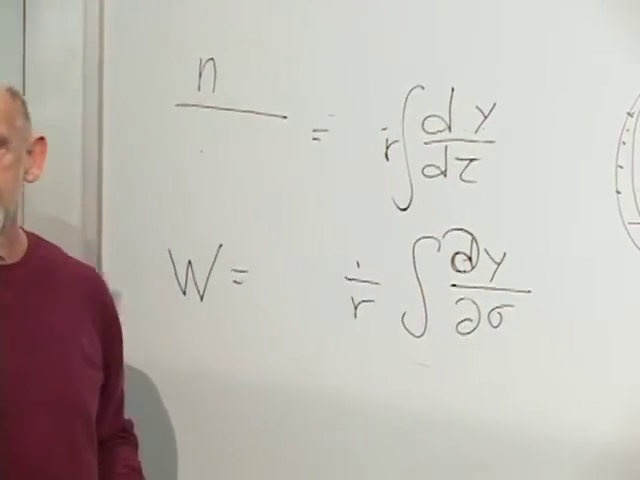
\includegraphics[width=0.72\textwidth]{lecture_10_figure_03.png}
  \medskip

  \begin{tikzpicture}[x=1cm,y=1cm,>=Latex]
    \draw[thick] (-4.0,0.3) circle (0.65);
    \draw[->,thick] (-4.55,0.58) arc (150:-145:0.65);
    \node at (-4.0,-0.65) {$w=+1$};
    \draw[thick] (-2.0,0.3) circle (0.65);
    \draw[->,thick] (-2.55,0.58) arc (150:-145:0.65);
    \node at (-2.0,-0.65) {$w=+1$};
    \node at (-3.0,0.3) {$+$};
    \draw[->,thick] (-1.0,0.3) -- (0.3,0.3);
    \draw[thick] (1.45,0.3) circle (0.78);
    \draw[thick] (1.45,0.3) circle (0.52);
    \draw[->,thick] (0.81,0.74) arc (145:-145:0.78);
    \node at (1.45,-0.78) {$w=+2$};
  \end{tikzpicture}
  \caption{Enrollamientos del mismo signo pueden reconectarse para formar una cuerda con el doble de enrollamiento. Cambia la conectividad, pero el enrollamiento total sigue siendo dos.}
  \lectureframe{00:16:40}
  \label{fig:l10-same-winding}
\end{figure}

Esta distinción se mantiene en todos los procesos permitidos. Un enrollamiento total de cien podría corresponder a una cuerda enrollada cien veces, a dos cuerdas enrolladas cincuenta veces cada una o a cien cuerdas enrolladas una vez. Las cuerdas pueden escindirse y unirse entre estas configuraciones, pero la suma con signo sigue siendo cien. La denotamos por \(w\in\mathbb Z\).

\section{Modos de momento y modos de enrollamiento}

La conservación por sí sola todavía no es dualidad. A continuación, compararemos las energías. Un estado que se mueve alrededor del círculo compacto tiene momento cuantizado
\begin{equation}
  p_Y=\frac{n}{R},
  \qquad n\in\mathbb Z.
  \label{eq:l10-compact-momentum}
\end{equation}
Para un estado en el que se puedan despreciar las demás contribuciones a la masa, el movimiento en la dimensión compacta contribuye \(E_{\rm mom}=|n|/R\). Los valores positivo y negativo de \(n\) indican sentidos opuestos del movimiento, mientras que la energía es positiva.

\begin{figure}[H]
  \centering
  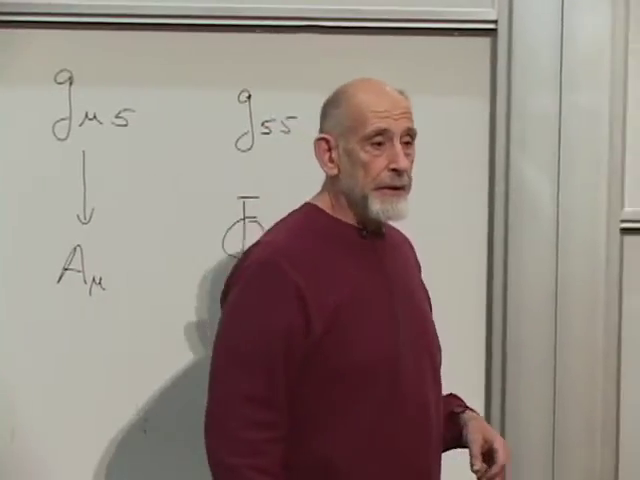
\includegraphics[width=0.72\textwidth]{lecture_10_figure_04.png}
  \caption{El número cuántico del momento compacto que aparece en la pizarra. En la clase, el momento se escribe esquemáticamente como una integral de la velocidad en la dirección compacta.}
  \lectureframe{00:21:30}
  \label{fig:l10-compact-momentum-board}
\end{figure}

Una cuerda enrollada \(|w|\) veces tiene longitud \(2\pi |w|R\). Con tensión fundamental de cuerda
\begin{equation}
  T_{\rm F}=\frac{1}{2\pi\alpha'},
\end{equation}
su energía de enrollamiento es
\begin{equation}
  E_{\rm wind}=T_{\rm F}(2\pi |w|R)
  =\frac{|w|R}{\alpha'}.
  \label{eq:l10-winding-energy}
\end{equation}
En las unidades de la clase \(\alpha'=1\), esto se reduce a \(E_{\rm wind}=|w|R\).

Las dos torres se comportan de manera opuesta cuando cambia el radio. Para \(R\gg
\sqrt{\alpha'}\), los niveles de momento están muy juntos y los de enrollamiento, muy separados. Para \(R\ll\sqrt{\alpha'}\), los niveles de momento están muy separados y los de enrollamiento, muy juntos.

\begin{figure}[H]
  \centering
  \begin{minipage}[t]{0.48\textwidth}
    \centering
    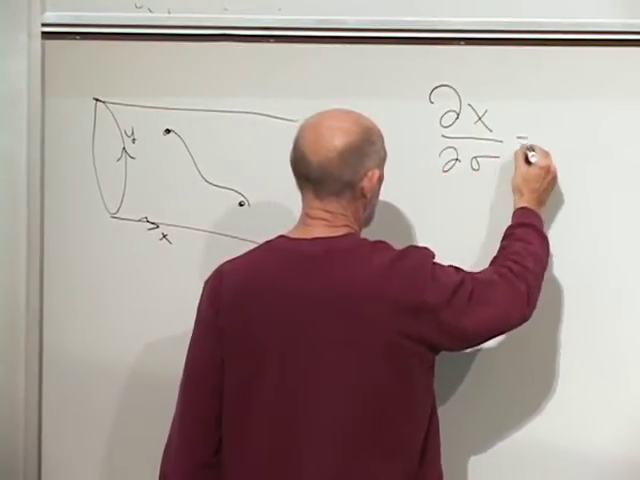
\includegraphics[width=\linewidth]{lecture_10_figure_05.png}
    \par\smallskip
    \textit{Radio compacto grande.}
  \end{minipage}\hfill
  \begin{minipage}[t]{0.48\textwidth}
    \centering
    \includegraphics[width=\linewidth]{lecture_10_figure_06.png}
    \par\smallskip
    \textit{Radio compacto pequeño.}
  \end{minipage}
  \caption{Las dos comparaciones espectrales de la pizarra. Las torres dispersas y densas intercambian sus papeles al invertir el radio.}
  \lectureframe{00:25:30--00:26:00}
  \label{fig:l10-dual-spectra-board}
\end{figure}

El esquema más claro es
\begin{figure}[H]
  \centering
  \begin{adjustbox}{max width=\linewidth}
  \begin{tikzpicture}[x=1cm,y=0.74cm,>=Latex]
    \node[font=\bfseries] at (-3.6,6.2) {$R\gg\sqrt{\alpha'}$};
    \draw[->] (-5.1,0) -- (-5.1,5.5) node[above] {$E$};
    \foreach \y in {0.4,1.0,1.6,2.2,2.8,3.4,4.0,4.6}
      \draw (-5.35,\y)--(-4.85,\y);
    \node[align=center] at (-4.25,5.15) {momentum\\dense};
    \draw[->] (-2.2,0) -- (-2.2,5.5) node[above] {$E$};
    \foreach \y in {0.4,2.4,4.4}
      \draw (-2.45,\y)--(-1.95,\y);
    \node[align=center] at (-1.35,5.15) {winding\\sparse};

    \node[font=\bfseries] at (3.6,6.2) {$R\ll\sqrt{\alpha'}$};
    \draw[->] (2.2,0) -- (2.2,5.5) node[above] {$E$};
    \foreach \y in {0.4,2.4,4.4}
      \draw (1.95,\y)--(2.45,\y);
    \node[align=center] at (3.05,5.15) {momentum\\sparse};
    \draw[->] (5.1,0) -- (5.1,5.5) node[above] {$E$};
    \foreach \y in {0.4,1.0,1.6,2.2,2.8,3.4,4.0,4.6}
      \draw (4.85,\y)--(5.35,\y);
    \node[align=center] at (5.95,5.15) {winding\\dense};
  \end{tikzpicture}
  \end{adjustbox}
  \caption{Reconstrucción del argumento basado en la separación entre niveles. El espectro completo de la cuerda no cambia cuando se intercambian el momento y el enrollamiento junto con \(R\leftrightarrow\alpha'/R\).}
  \label{fig:l10-dual-spectra-redraw}
\end{figure}

Supongamos que alguien recibe uno de estos espectros sin que le digan cómo se obtuvo. ¿Es la torre de niveles muy juntos el momento en un círculo grande o el enrollamiento en uno pequeño? El espectro por sí solo no permite saberlo. La teoría de cuerdas afirma algo más fuerte: tampoco los elementos de matriz de dispersión permiten distinguirlos. Las dos descripciones son exactamente equivalentes bajo
\begin{equation}
  n\longleftrightarrow w,
  \qquad
  R\longleftrightarrow \widetilde R=\frac{\alpha'}{R}.
  \label{eq:l10-radius-duality}
\end{equation}
El punto fijo es
\begin{equation}
  R=\sqrt{\alpha'},
  \label{eq:l10-self-dual-radius}
\end{equation}
o \(R=1\) en las unidades de la clase. En ese radio pueden volverse sin masa estados adicionales y se realza la simetría gauge.

\begin{classroomqa}
\audiencequestion{¿El enrollamiento es solo una conveniencia matemática para reescribir el espectro? \lecturetimestamp{00:27:33}}
\lecturerresponse{No. El enrollamiento etiqueta sectores reales del espacio de Hilbert de la cuerda cerrada, y esos sectores participan en las interacciones. La palabra ``dualidad'' significa que las descripciones en términos de momento y de enrollamiento son coordenadas distintas para una misma física, no que uno de los sectores sea un recurso mnemotécnico opcional para representar el otro.}
\end{classroomqa}

\begin{classroomqa}
\audiencequestion{¿Hay algún radio que se transforme en sí mismo?
\lecturetimestamp{00:27:58}}
\lecturerresponse{Sí. El valor autodual es
\(R=\sqrt{\alpha'}\), que corresponde a \(R=1\) en las unidades usadas en la pizarra. Allí coinciden las dos torres y el espectro presenta una simetría realzada.}
\end{classroomqa}

\section{La forma de la dualidad en la hoja de mundo}

El argumento espectral es sugerente, pero la hoja de mundo hace más precisa la correspondencia. En el gauge conforme, el momento conjugado a \(Y\) es proporcional a \(\partial_\tau Y\). Así, el momento compacto total tiene la forma
\begin{equation}
  P_Y=\frac{1}{2\pi\alpha'}
      \int_0^{2\pi}d\sigma\,\partial_\tau Y.
  \label{eq:l10-worldsheet-momentum}
\end{equation}
El número de enrollamiento es
\begin{equation}
  w=\frac{1}{2\pi R}
      \int_0^{2\pi}d\sigma\,\partial_\sigma Y
   =\frac{Y(2\pi)-Y(0)}{2\pi R}.
  \label{eq:l10-worldsheet-winding}
\end{equation}

\begin{classroomqa}
\audiencequestion{¿Por qué no se anula la integral de una derivada al recorrer la cuerda cerrada? \lecturetimestamp{00:32:33}}
\lecturerresponse{Porque \(Y\) es una coordenada periódica del espacio objetivo, no una función real univaluada en el círculo de coordenada \(\sigma\). El punto de la hoja de mundo \(\sigma=2\pi\) es el mismo que \(\sigma=0\), pero un levantamiento de la aplicación de inmersión a la recta recubridora cambia en \(2\pi wR\). La integral de \(\partial_\sigma Y\) mide ese desplazamiento.}
\end{classroomqa}

\begin{figure}[H]
  \centering
  \includegraphics[width=0.76\textwidth]{lecture_10_figure_07.png}
  \caption{Las integrales de momento y de enrollamiento, una vez completadas ambas expresiones en la pizarra. En la normalización de la clase se omiten los factores comunes \(2\pi\) y \(\alpha'\).}
  \lectureframe{00:33:25}
  \label{fig:l10-momentum-winding-integrals}
\end{figure}

Para una cuerda enrollada una vez,
\begin{equation}
  Y(\tau,\sigma+2\pi)=Y(\tau,\sigma)+2\pi R.
\end{equation}
Para un enrollamiento \(w\), el desplazamiento del lado derecho es \(2\pi wR\). La ecuación \eqref{eq:l10-worldsheet-winding} cuenta entonces exactamente el enrollamiento. Esta es la formulación precisa de la abreviatura de la pizarra \(w\sim R^{-1}\int
d\sigma\,\partial_\sigma Y\).

Por tanto, la formulación de la dualidad T en la hoja de mundo es
\begin{equation}
  \partial_\tau Y\longleftrightarrow
  \partial_\sigma \widetilde Y,
  \qquad
  \partial_\sigma Y\longleftrightarrow
  \partial_\tau \widetilde Y,
  \label{eq:l10-derivative-duality}
\end{equation}
donde el momento en \(Y\) se convierte en enrollamiento en la coordenada dual \(\widetilde Y\), y viceversa.

\begin{classroomqa}
\audiencequestion{¿Significa esto que las coordenadas de la hoja de mundo \(\tau\) y \(\sigma\) están relacionadas o se intercambian entre sí?
\lecturetimestamp{00:34:39}}
\lecturerresponse{No. La dualidad T transforma soluciones e intercambia derivadas específicas de la coordenada compacta del espacio objetivo. No identifica la coordenada temporal de la hoja de mundo con su coordenada espacial.}
\end{classroomqa}

\section{Por qué no se pueden evitar los estados con enrollamiento}

Cabe preguntarse por qué una cuerda llegaría a estar enrollada si existe un estado no enrollado. Una cuerda no elige su estado por preferencia. La energía suministrada en una colisión la estira. Una cuerda suficientemente energética y muy deformada puede reconectarse y dar lugar a dos cuerdas con enrollamientos opuestos. Su enrollamiento total sigue siendo cero, pero después de la escisión las dos cuerdas pueden separarse. Una de ellas puede alejarse mucho, y dejar a un observador con una cuerda aparentemente aislada y enrollada.

\begin{figure}[H]
  \centering
  \includegraphics[width=0.76\textwidth]{lecture_10_figure_08.png}
  \caption{Una configuración muy estirada con enrollamiento neto nulo, de la que pueden separarse cuerdas con enrollamientos opuestos tras la reconexión.}
  \lectureframe{00:36:15}
  \label{fig:l10-winding-pair-production}
\end{figure}

El umbral de energía viene determinado por la energía de enrollamiento. En un círculo grande, hace falta una energía de colisión elevada para estirar la cuerda lo suficiente como para que dé una vuelta alrededor de la dimensión compacta. Sin embargo, por encima del umbral no se puede prohibir la producción de pares de cuerdas enrolladas y anti-enrolladas--. La analogía es la producción de pares de electrones-- y positrones en colisiones de fotones. La carga eléctrica total sigue siendo cero, pero las partículas cargadas están presentes y pueden separarse. La conservación del enrollamiento funciona del mismo modo.

Esta analogía es más que una manera de hablar. El momento compacto y el enrollamiento se comportan como dos números cuánticos de carga distintos. En la descripción reducida correspondiente, las cargas del mismo signo se repelen y las de signo opuesto se atraen. Por tanto, debemos preguntar cuáles son los dos campos vectoriales que median esas fuerzas.

\section{Carga de momento a partir de la gravedad en cinco dimensiones}

Empecemos con la gravedad en cinco dimensiones. Sean los índices mayúsculos \(M,N\), que recorren las cuatro direcciones ordinarias del espacio-tiempo y la quinta dirección compacta. La métrica se descompone como
\begin{equation}
  G_{MN}\quad\longrightarrow\quad
  \bigl\{G_{\mu\nu},\,G_{\mu5},\,G_{55}\bigr\}.
  \label{eq:l10-metric-decomposition}
\end{equation}
La componente simétrica \(G_{5\mu}\) no contiene información nueva respecto de \(G_{\mu5}\).

\begin{figure}[H]
  \centering
  \includegraphics[width=0.74\textwidth]{lecture_10_figure_09.png}
  \caption{Los grupos independientes de componentes de la métrica en cinco dimensiones: \(G_{\mu\nu}\), \(G_{\mu5}\) y \(G_{55}\).}
  \lectureframe{00:44:05}
  \label{fig:l10-metric-components}
\end{figure}

Desde el punto de vista de cuatro dimensiones,
\begin{align}
  G_{\mu\nu} &\quad\hbox{is a spacetime metric},\\
  G_{\mu5} &\equiv A_\mu\quad\hbox{is a vector field},\\
  G_{55} &\equiv e^{2\varphi}\quad\hbox{is a scalar modulus}.
  \label{eq:l10-four-dimensional-fields}
\end{align}
El escalar \(\varphi\) mide el tamaño de la dimensión compacta. Puede variar suavemente a lo largo del espacio-tiempo ordinario, de modo que las ondas de \(\varphi\) son ondas en el radio de la quinta dimensión.

\begin{figure}[H]
  \centering
  \includegraphics[width=0.74\textwidth]{lecture_10_figure_10.png}
  \caption{En la pizarra se identifica \(G_{\mu5}\) con un vector \(A_\mu\) y \(G_{55}\) con un escalar \(\Phi\).}
  \lectureframe{00:47:40}
  \label{fig:l10-vector-and-radius-modulus}
\end{figure}

La fuente de una componente gravitatoria mixta es un flujo de momento mixto. En particular, el momento en la quinta dirección es fuente de \(G_{\mu5}\). Por tanto, un observador en cuatro dimensiones interpreta el entero \(n\) como una carga eléctrica acoplada a \(A_\mu\). Este es el mecanismo de Kaluza--Klein: lo que es momento en la geometría de dimensiones superiores se convierte en carga en la teoría de campos de dimensiones inferiores.

\editorialnote{En la clase se llama de manera informal \(G_{55}\) «``dilatón''» al escalar. En esta reducción es, en concreto, el módulo del radio. El dilatón de la cuerda en diez dimensiones, que controla el acoplamiento de cuerda, es un campo distinto, aunque ciertas combinaciones escalares de dimensiones inferiores pueden mezclarse al cambiar de marco y bajo dualidad.}

\begin{classroomqa}
\audiencequestion{¿El escalar \(\varphi\) es proporcional al entero de momento \(n\)? \lecturetimestamp{00:48:43}}
\lecturerresponse{No. El entero \(n\) etiqueta un estado cuantizado y actúa como carga. El escalar \(\varphi(x)\) es un campo continuo que determina el tamaño local de la compactificación. Puede variar de un lugar a otro; no es en sí mismo un entero.}
\end{classroomqa}

\section{El segundo campo vectorial y la carga de enrollamiento}

El enrollamiento también se comporta como una carga, pero no puede acoplarse al mismo vector de la misma manera. Para encontrar el segundo vector, volvamos a las primeras excitaciones de la cuerda cerrada. Una cuerda cerrada tiene modos de oscilador que se propagan hacia la izquierda y hacia la derecha. Los estados físicos satisfacen la condición de igualación de niveles: los niveles totales de excitación izquierda y derecha deben coincidir.

En la teoría bosónica, el estado no excitado es el taquión. Un solo oscilador de movimiento a la izquierda o a la derecha incumpliría la condición de igualación de niveles. Por tanto, el primer estado sin masa permitido contiene un oscilador de cada tipo,
\begin{equation}
  \alpha_{-1}^{I}\widetilde\alpha_{-1}^{J}\ket{0;k}.
  \label{eq:l10-first-massless-state}
\end{equation}
Los índices \(I,J\) recorren las direcciones espaciales transversales, incluida la dirección compacta. Si un índice corresponde a una dirección ordinaria y el otro a \(5\), hay dos estados de oscilador de tipo vectorial,
\begin{equation}
  \alpha_{-1}^{\mu}\widetilde\alpha_{-1}^{5}\ket{0;k},
  \qquad
  \alpha_{-1}^{5}\widetilde\alpha_{-1}^{\mu}\ket{0;k}.
  \label{eq:l10-two-vector-states}
\end{equation}

\begin{figure}[H]
  \centering
  \includegraphics[width=0.76\textwidth]{lecture_10_figure_11.png}
  \caption{Los dos órdenes de los osciladores izquierdo-- y derecho que dan lugar a estados vectoriales en cuatro dimensiones cuando una polarización apunta en la dirección compacta.}
  \lectureframe{00:58:20}
  \label{fig:l10-two-vector-states-board}
\end{figure}

Sus combinaciones simétrica y antisimétrica pertenecen a campos distintos del espacio-tiempo:
\begin{align}
  \alpha_{-1}^{(\mu}\widetilde\alpha_{-1}^{5)}\ket{0;k}
    &\longleftrightarrow G_{\mu5},\\
  \alpha_{-1}^{[\mu}\widetilde\alpha_{-1}^{5]}\ket{0;k}
    &\longleftrightarrow B_{\mu5}.
  \label{eq:l10-g-and-b-vectors}
\end{align}
El primero es el vector de Kaluza--Klein, cuya fuente es el momento compacto. El segundo desciende del campo antisimétrico de Kalb--Ramond y tiene como fuente el enrollamiento de la cuerda. Así, la teoría reducida contiene dos campos de tipo fotónico, uno para cada sector de carga.

Si ambos índices del oscilador apuntan en la dirección compacta, el estado es un escalar asociado al módulo de compactificación. Si ambos corresponden a direcciones transversales ordinarias, la parte simétrica sin traza es el gravitón, la parte antisimétrica es \(B_{\mu\nu}\) y la traza contribuye a un sector escalar.

\begin{classroomqa}
\audiencequestion{¿Cuál de estos estados es el singlete y cuál el triplete? \lecturetimestamp{01:00:21}}
\lecturerresponse{Esa clasificación no resulta útil aquí. Ambos estados mixtos se transforman como vectores en cuatro dimensiones. Su suma y su diferencia separan la polarización simétrica de la métrica de la polarización antisimétrica del campo \(B\). En cambio, el estado con dos índices compactos es un escalar en cuatro dimensiones.}
\end{classroomqa}

El diccionario completo al que llegamos antes de la pausa es
\begin{equation}
  \boxed{
  \begin{gathered}
    n\leftrightarrow w,
    \qquad
    R\leftrightarrow\dfrac{\alpha'}{R},\\
    \partial_\tau Y\leftrightarrow\partial_\sigma\widetilde Y,
    \qquad
    G_{\mu5}\leftrightarrow B_{\mu5}.
  \end{gathered}}
  \label{eq:l10-complete-t-duality-map}
\end{equation}

\begin{figure}[H]
  \centering
  \includegraphics[width=0.72\textwidth]{lecture_10_figure_12.png}
  \caption{Resumen de la correspondencia de dualidad T en la pizarra: se intercambian el momento y el enrollamiento, el radio y su inverso, las derivadas de la hoja de mundo y los dos campos vectoriales. El profesor oculta parcialmente la última línea, que por ello se incluye explícitamente en la ecuación \eqref{eq:l10-complete-t-duality-map}.}
  \lectureframe{01:02:20}
  \label{fig:l10-t-duality-map-board}
\end{figure}

Esta construcción no debe confundirse con la afirmación de que todos los campos enumerados ya se hayan identificado en el espectro observado de partículas. En este punto, es una consecuencia matemática de la teoría de cuerdas compactificada. Hay muchas propuestas para conectar estas estructuras con la fenomenología, pero ese no es el problema que resuelve esta clase.

\section{Las cuerdas abiertas cambian la pregunta}

Después de la pausa, retomamos el análisis con las cuerdas abiertas. Una cuerda cerrada puede tener un enrollamiento estable porque no tiene extremos por los que este pueda escabullirse. Una cuerda abierta tiene extremos y, por tanto, no posee un número de enrollamiento análogo protegido topológicamente. Sin embargo, la dualidad T es una simetría exacta de la teoría. ¿Qué hace esta simetría con una cuerda abierta?

Para un extremo que se mueve libremente, la variación de la acción de la cuerda da una condición de contorno de Neumann. En la geometría sencilla \((X,Y)\),
\begin{equation}
  \left.\partial_\sigma X\right|_{\partial\Sigma}=0,
  \qquad
  \left.\partial_\sigma Y\right|_{\partial\Sigma}=0.
  \label{eq:l10-neumann-boundary}
\end{equation}
La imagen mecánica es sencilla. Consideremos la cuerda como una cadena de elementos de masa cada vez más pequeños. Una fuerza tangencial no nula sobre el último elemento le produciría una aceleración que diverge cuando su masa tiende a cero. Por tanto, un extremo libre se ajusta hasta que la tensión neta en el extremo se anula. Otra persona podría sujetar el extremo fijo y ejercer la fuerza necesaria, pero entonces el extremo dejaría de ser libre.

\begin{figure}[H]
  \centering
  \includegraphics[width=0.76\textwidth]{lecture_10_figure_13.png}
  \caption{La cuerda abierta y sus condiciones de contorno de Neumann completas en los extremos, \(\partial_\sigma X=\partial_\sigma Y=0\).}
  \lectureframe{01:09:20}
  \label{fig:l10-neumann-board}
\end{figure}

Dualicemos ahora únicamente la coordenada compacta \(Y\). La coordenada no compacta \(X\) no cambia. La ecuación \eqref{eq:l10-derivative-duality} transforma la segunda condición de Neumann en
\begin{equation}
  \left.\partial_\tau\widetilde Y\right|_{\partial\Sigma}=0.
  \label{eq:l10-dirichlet-time-derivative}
\end{equation}
Por tanto, la posición del extremo en la dirección compacta dual no depende del tiempo,
\begin{equation}
  \left.\widetilde Y\right|_{\partial\Sigma}=Y_0.
  \label{eq:l10-dirichlet-boundary}
\end{equation}
Esta es una condición de contorno de Dirichlet.

\begin{figure}[H]
  \centering
  \includegraphics[width=0.76\textwidth]{lecture_10_figure_14.png}
  \medskip

  \begin{adjustbox}{max width=\linewidth}
  \begin{tikzpicture}[x=1cm,y=1cm,>=Latex]
    \node[align=center] at (-3.5,0.8)
      {Neumann\\\(\left.\partial_\sigma Y\right|_{\partial\Sigma}=0\)};
    \draw[->,thick] (-1.7,0.8) -- (1.3,0.8)
      node[midway,above] {$T_Y$};
    \node[align=center] at (3.4,0.8)
      {Dirichlet\\\(\left.\partial_\tau\widetilde Y\right|_{\partial\Sigma}=0\)};
    \node[align=center] at (3.4,-0.5)
      {\(\widetilde Y(\tau)=Y_0\) at each endpoint};
  \end{tikzpicture}
  \end{adjustbox}
  \caption{La condición de contorno completa del extremo dual en la pizarra y su reconstrucción lógica clara. La dualidad T transforma la libertad en la dirección compacta en una posición fija del extremo en la dirección dual.}
  \lectureframe{01:12:35}
  \label{fig:l10-neumann-to-dirichlet}
\end{figure}

\begin{classroomqa}
\audiencequestion{¿Por qué significa la condición dual que el extremo está fijo? \lecturetimestamp{01:12:39}}
\lecturerresponse{Porque \(\partial_\tau\widetilde Y=0\) es una velocidad nula en la dirección dualizada. Dondequiera que comience el extremo en \(\widetilde Y\), allí permanecerá. Sus coordenadas en las direcciones paralelas a las no dualizadas siguen siendo libres.}
\end{classroomqa}

\section{El objeto que sujeta el extremo es una D-brana}

Si un extremo está fijo, algo debe poder mantenerlo allí. Por tanto, la dualidad T exacta exige un objeto nuevo sobre el que puedan terminar las cuerdas abiertas. Ese objeto es una D-brana. La letra \(D\) representa Dirichlet, no la dimensión del objeto. En el aparte histórico de la clase se señala que estos objetos podrían haberse llamado en honor de Joseph Polchinski, cuyo análisis hizo innegable su papel dinámico; sin embargo, el término ya establecido «``p-brana''» hacía de Dirichlet el nombre más natural.

Una brana de tipo \(p\) tiene \(p\) dimensiones espaciales. Una cuerda es una brana de una dimensión, una membrana es una brana de dos dimensiones y un objeto extenso tridimensional es una brana de tres dimensiones. Una D\(p\)-brana es una brana de tipo \(p\) en la que los extremos de las cuerdas fundamentales satisfacen condiciones de Dirichlet en las direcciones transversales y condiciones de Neumann en las direcciones tangentes a la brana.

Nada en el argumento de dualidad señala un valor particular de \(Y_0\); por tanto, la D-brana no puede ser un soporte rígido clavado en un punto preferente del universo. Debe poder moverse. La relatividad también prohíbe los cuerpos extensos absolutamente rígidos, así que una D-brana puede fluctuar y curvarse. La brana plana y sencilla dibujada en la pizarra es su configuración de equilibrio, no una restricción a su dinámica.

\begin{classroomqa}
\audiencequestion{¿Deben los dos extremos de una cuerda abierta tener el mismo valor fijo de la coordenada dual? \lecturetimestamp{01:14:55}}
\lecturerresponse{No necesariamente. Ambos extremos pueden estar sobre la misma D-brana, en cuyo caso comparten la posición transversal de esa brana. También pueden estar sobre dos D-branas distintas, situadas en posiciones transversales diferentes; entonces la cuerda se extiende entre ellas. La propia brana puede fluctuar y curvarse, de modo que el lugar geométrico de los extremos no tiene por qué seguir siendo un plano perfectamente llano.}
\end{classroomqa}

\section{Cómo contar las dimensiones de una D-brana}

La teoría de supercuerdas en diez dimensiones tiene nueve dimensiones espaciales. Supongamos que la dualidad T impone una condición de Dirichlet en una dirección espacial. El extremo aún puede moverse libremente en las otras ocho, de modo que su lugar geométrico permitido es una D8-brana de ocho dimensiones. Cada condición de Dirichlet independiente adicional elimina una dirección de movimiento del extremo. Si se fijan \(k\) coordenadas espaciales, entonces
\begin{equation}
  p=9-k.
  \label{eq:l10-dp-counting}
\end{equation}

La mesa ilustra la misma cuenta en tres dimensiones. Si se fija la coordenada vertical, la yema de un dedo puede moverse sobre una mesa bidimensional. Si se fija una segunda coordenada, solo puede moverse a lo largo de una línea. Si se fijan las tres, queda confinada a un punto.

\begin{figure}[H]
  \centering
  \begin{adjustbox}{max width=\linewidth}
  \begin{tikzpicture}[x=1.05cm,y=1cm,>=Latex]
    \draw[fill=blue!8] (-5.5,-0.7) -- (-2.5,-0.7) -- (-1.7,0.2)
      -- (-4.7,0.2) -- cycle;
    \node at (-3.6,-1.15) {one constraint: sheet};
    \draw[very thick,blue!60!black] (-0.9,-0.25) -- (1.3,-0.25);
    \node at (0.2,-1.15) {two constraints: line};
    \fill[blue!70!black] (4.1,-0.25) circle (0.09);
    \node at (4.1,-1.15) {three constraints: point};
    \draw[->] (-1.45,0.95) -- (-0.75,0.95);
    \draw[->] (2.25,0.95) -- (2.95,0.95);
    \node at (0.35,1.35) {each Dirichlet condition lowers \(p\) by one};
  \end{tikzpicture}
  \end{adjustbox}
  \caption{El argumento de recuento de dimensiones ilustrado en la mesa. Una D\(p\)-brana es el lugar geométrico en el que los extremos pueden moverse libremente.}
  \label{fig:l10-dp-counting-redraw}
\end{figure}

Las dualidades sucesivas generan D8-, D7-, D6-branas y así sucesivamente, hasta llegar a una D0-brana, que es puntual en el espacio. Si no se fija ninguna dirección espacial, una D9-brana ocupa las nueve dimensiones espaciales y las cuerdas abiertas ordinarias pueden moverse por todas partes. En la clase se mencionan brevemente las D\((-1)\)-branas; están localizadas en el espacio-tiempo euclídeo y se comportan como instantones, no como partículas ordinarias que se propagan en el tiempo.

\editorialnote{La escala de dimensiones es una afirmación sobre las teorías de tipo II consideradas en conjunto. Las D\(p\)-branas BPS estables tienen valor par de \(p\) en la teoría de tipo IIA y valor impar de \(p\) en la teoría de tipo IIB. La dualidad T a lo largo de un círculo cambia \(p\) en una unidad e intercambia simultáneamente las teorías de tipo IIA y de tipo IIB.}

\begin{classroomqa}
\audiencequestion{Si solo hay seis dimensiones compactas, ¿debería empezar el recuento restando a partir de seis en lugar de nueve? \lecturetimestamp{01:20:49}}
\lecturerresponse{La derivación elemental aplica la dualidad T a las direcciones compactas, pero el círculo dual se vuelve arbitrariamente grande cuando el círculo original se hace arbitrariamente pequeño. En ese límite, es efectivamente no compacto. Por tanto, las branas resultantes pueden extenderse a lo largo de direcciones o ser transversales a ellas, aunque a escalas accesibles parezcan no compactas. La dimensión \(p\) cuenta todas las direcciones espaciales tangentes a la brana, no solo las compactas que se usan en una derivación concreta.}
\end{classroomqa}

Una D0-brana es un nuevo tipo de partícula. Una cuerda abierta puede ir de una D0-brana a otra, regresar a la misma D0-brana o extenderse hacia una brana muy distante. Si uno de sus extremos llegara literalmente al infinito espacial, la cuerda tendría longitud infinita y, por tanto, energía infinita; así que la opción físicamente útil consiste en situar el otro extremo en otro objeto.

El siguiente caso, una D1-brana, también tiene forma de cuerda, pero no es la cuerda fundamental con la que empezamos. Puede curvarse y cerrarse sobre sí misma, y las cuerdas fundamentales pueden terminar en ella. Su tensión depende de manera distinta del acoplamiento de cuerdas:
\begin{equation}
  T_{\rm D1}=\frac{1}{2\pi\alpha' g_s},
  \qquad
  T_{\rm F1}=\frac{1}{2\pi\alpha'}.
  \label{eq:l10-dstring-tension}
\end{equation}
A acoplamiento débil \(g_s\ll1\), la cuerda D es mucho más pesada que la cuerda fundamental, lo que explica por qué aparece primero como un ancla masiva.

\begin{figure}[H]
  \centering
  \includegraphics[width=0.76\textwidth]{lecture_10_figure_15.png}
  \caption{La D1-brana de la pizarra: un objeto unidimensional flexible, distinto de las cuerdas fundamentales que pueden terminar en ella.}
  \lectureframe{01:24:20}
  \label{fig:l10-d1-brane}
\end{figure}

\begin{classroomqa}
\audiencequestion{¿Actúa la dualidad T sobre las D-branas además de sobre las cuerdas? \lecturetimestamp{01:25:35}}
\lecturerresponse{Sí. Una dualidad T paralela a una D\(p\)-brana reduce su dimensión a D\((p-1)\), mientras que una dualidad T transversal a ella aumenta su dimensión a D\((p+1)\). Las branas forman parte del diccionario de dualidad; no son soportes externos que esta deje intactos.}
\end{classroomqa}

\begin{classroomqa}
\audiencequestion{¿Pueden seguir siendo compactas las direcciones tangentes a una brana?
\lecturetimestamp{01:27:25}}
\lecturerresponse{Sí. ``Tangencial'' y ``compacta'' responden a preguntas distintas. Una dirección puede extenderse a lo largo de la brana y aun así cerrarse formando un círculo; también puede ser no compacta. Para el extremo, lo que importa es si la condición de contorno en esa dirección es de Neumann o de Dirichlet.}
\end{classroomqa}

Una D2-brana es una lámina similar a una membrana. Una D3-brana tiene tres dimensiones espaciales. En un espacio-tiempo genuinamente de dimensiones superiores, una D3-brana es un subespacio tridimensional, no todo el espacio, aunque los observadores confinados a ella puedan experimentarla como la totalidad de su mundo espacial.

\begin{figure}[H]
  \centering
  \includegraphics[width=0.76\textwidth]{lecture_10_figure_16.png}
  \caption{Una D2-brana representada como una lámina sobre la que pueden moverse los extremos de las cuerdas.}
  \lectureframe{01:27:55}
  \label{fig:l10-d2-brane}
\end{figure}

La derivación que se presenta aquí es deliberadamente esquemática. Por sí sola, no demuestra que la teoría de cuerdas describa la naturaleza. Sin embargo, dentro de la teoría de cuerdas hay numerosas comprobaciones de consistencia: las dualidades, los cálculos cuánticos y los resultados matemáticos apuntan a que las D-branas son objetos dinámicos reales.

\section{Las cuerdas abiertas se convierten en campos en una brana}

Tomemos una D2-brana vacía y coloquemos en ella cuerdas abiertas cortas. Cada extremo está confinado a la lámina, de modo que toda la excitación de baja energía se mueve a lo largo de ella. Dos cuerdas orientadas cuyos extremos adyacentes tengan flechas compatibles pueden unirse. Más adelante, la cuerda resultante puede volver a dividirse. Interpretados como historias de partículas, estos procesos son los vértices de los diagramas de Feynman: entran dos partículas, se propaga una excitación intermedia y salen dos partículas.

\begin{figure}[H]
  \centering
  \includegraphics[width=0.76\textwidth]{lecture_10_figure_17.png}
  \caption{Cuerdas abiertas orientadas sobre una D2-brana que se unen mediante extremos compatibles. A baja energía, el proceso se interpreta como una interacción de teoría de campos en la brana.}
  \lectureframe{01:29:55}
  \label{fig:l10-open-strings-on-brane}
\end{figure}

A energías muy inferiores a la escala de cuerdas, no se excita la torre de modos vibracionales internos. El estado restante de cuerda abierta, que no tiene masa, es un campo vectorial en el volumen de mundo de la brana. Para una sola brana, se trata de un campo de gauge abeliano \(U(1)\), análogo en la brana al electromagnetismo. El campo no se propaga por todo el volumen de diez dimensiones; sus cuantos son cuerdas abiertas cuyos extremos los mantienen en la brana.

\section{Una pila de branas produce color no abeliano}

Ahora coloquemos varias branas paralelas cerca unas de otras. Para tres branas, llamémoslas Roja, Verde y Azul. Una cuerda orientada tiene un par ordenado de etiquetas en sus extremos: puede ir de Roja a Verde, de Verde a Azul, de Roja a Roja, etcétera. Con \(N\) branas, los estados de cuerda abierta sin masa pueden organizarse como una matriz \(N\times N\)
\begin{equation}
  A_\mu{}^{i}{}_{j},
  \qquad i,j=1,\ldots,N.
  \label{eq:l10-chan-paton-matrix}
\end{equation}
Estas son las etiquetas de Chan--Paton de una teoría de gauge \(U(N)\).

\begin{figure}[H]
  \centering
  \includegraphics[width=0.76\textwidth]{lecture_10_figure_18.png}
  \medskip

  \begin{adjustbox}{max width=\linewidth}
  \begin{tikzpicture}[x=1cm,y=1cm,>=Latex]
    \draw[very thick,red!70!black] (-4.8,2.0)--(4.8,2.0);
    \draw[very thick,green!55!black] (-4.8,0.8)--(4.8,0.8);
    \draw[very thick,blue!70!black] (-4.8,-0.4)--(4.8,-0.4);
    \node[left] at (-4.8,2.0) {Red};
    \node[left] at (-4.8,0.8) {Green};
    \node[left] at (-4.8,-0.4) {Blue};
    \draw[->,thick] (-3.4,2.0) .. controls (-2.8,1.35) and (-2.3,1.15)
      .. (-1.7,0.8);
    \node at (-2.7,1.05) {$R\!G$};
    \draw[->,thick] (-0.6,0.8) .. controls (0.0,0.25) and (0.6,-0.05)
      .. (1.2,-0.4);
    \node at (0.1,0.0) {$G\!B$};
    \draw[->,thick] (2.1,2.0) .. controls (2.9,2.55) and (3.8,2.55)
      .. (4.3,2.0);
    \node at (3.2,2.65) {$R\!R$};
  \end{tikzpicture}
  \end{adjustbox}
  \caption{Tres branas paralelas en la pizarra y una reconstrucción clara de las etiquetas ordenadas de los extremos que llevan las cuerdas que las conectan.}
  \lectureframe{01:33:15}
  \label{fig:l10-three-brane-stack}
\end{figure}

\begin{classroomqa}
\audiencequestion{¿Puede realmente una cuerda ir de la brana Roja a la brana Verde sin que se lo impidan los otros trazos del dibujo? \lecturetimestamp{01:35:07}}
\lecturerresponse{Sí. Las branas están inmersas en un espacio de dimensiones superiores. El dibujo bidimensional de la pizarra es solo una proyección, así que una cuerda puede pasar alrededor de otra línea proyectada desplazándose en una dirección transversal.}
\end{classroomqa}

\begin{classroomqa}
\audiencequestion{¿Es necesario que una cuerda Roja--Verde se combine con una cuerda Verde--Azul para convertirse en una Roja--Azul? \lecturetimestamp{01:35:39}}
\lecturerresponse{Esa es la regla básica de unión local. Los extremos compatibles se encuentran y los dos segmentos se convierten en una sola cuerda cuyos extremos libres conservan las etiquetas Roja y Azul. Los procesos más elaborados se construyen repitiendo la misma operación.}
\end{classroomqa}

La regla de unión es la multiplicación de matrices llevada a la geometría. Una cuerda Roja--Verde puede unirse con una cuerda Verde--Azul porque el extremo Verde de una es compatible con el extremo Verde de la otra. El resultado es una cuerda Roja--Azul:
\begin{equation}
  (R,G)\circ(G,B)\longrightarrow(R,B).
  \label{eq:l10-color-composition}
\end{equation}
El índice repetido se contrae y desaparece internamente. Esta es la misma estructura de índices que aparece en un vértice de interacción de Yang--Mills.

\begin{figure}[H]
  \centering
  \includegraphics[width=0.76\textwidth]{lecture_10_figure_19.png}
  \caption{Unión de cuerdas abiertas en una pila. La orientación de los extremos impone la misma composición de índices ordenados que se usa en los campos de gauge no abelianos.}
  \lectureframe{01:36:30}
  \label{fig:l10-color-joining-board}
\end{figure}

Para tres branas coincidentes, el grupo de gauge completo de las cuerdas abiertas es \(U(3)\), con nueve estados vectoriales. Su álgebra se descompone así:
\begin{equation}
  \mathfrak u(3)=\mathfrak{su}(3)\oplus\mathfrak u(1).
  \label{eq:l10-u3-decomposition}
\end{equation}
Las ocho combinaciones sin traza tienen la estructura de color de los gluones de la QCD, mientras que el \(U(1)\) diagonal del centro de masas es un campo abeliano independiente.

\editorialnote{La clase describe una de las nueve combinaciones de pares de color como algo que puede desprenderse y desaparecer, dejando así ocho gluones. La afirmación precisa sobre las D-branas es que una pila de tres branas coincidentes da \(U(3)\), no solo \(SU(3)\). Para obtener el octete de la QCD hay que separar, proyectar o desacoplar de algún otro modo el \(U(1)\) diagonal. La imagen de la clase motiva correctamente los índices de color ordenados, pero no constituye una derivación completa de la QCD.}

La materia similar a los quarks lleva un solo índice de color. En la imagen de las branas, la representa una cuerda con un extremo en la pila de color y el otro en una brana distinta y distante. Respecto de la pila de color, solo un extremo es visible como etiqueta de color. Al invertir la orientación se obtiene la antipartícula. Una cuerda similar a un quark y otra similar a un antiquark, con extremos compatibles, pueden unirse y separarse de la pila de color; dos cuerdas orientadas de la misma manera y similares a quarks no pueden aniquilarse de ese modo.

Las teorías resultantes de baja energía suelen ser teorías supersimétricas de Yang--Mills, con materia adicional determinada por las branas y sus intersecciones. Se parecen lo bastante a la QCD como para esclarecer la dinámica no abeliana, pero no son automáticamente el modelo estándar. Con una sola brana, la misma construcción se reduce a una teoría \(U(1)\): las cuerdas cortas entre branas--branas son similares a fotones, mientras que las cuerdas orientadas que llegan a un segundo sector desempeñan el papel de las cargas eléctricas positivas y negativas.

\section{Las cuerdas D terminan como monopolos magnéticos}

Ahora hay dos tipos de objetos con forma de cuerda en este relato. La cuerda fundamental, o cuerda F, transporta flujo eléctrico en una D3-brana. La D1-brana, o cuerda D, es mucho más pesada a acoplamiento débil. Una cuerda D también puede terminar en una D3-brana. Su extremo no tiene carga eléctrica respecto del campo de gauge del volumen de mundo; tiene carga magnética. Desde la perspectiva de los observadores en la D3-brana, el extremo es un monopolo magnético.

\begin{figure}[H]
  \centering
  \includegraphics[width=0.76\textwidth]{lecture_10_figure_20.png}
  \medskip

  \begin{adjustbox}{max width=\linewidth}
  \begin{tikzpicture}[x=1cm,y=1cm,>=Latex]
    \draw[fill=blue!7] (-3.8,-0.5)--(2.6,-0.5)--(3.6,0.35)--(-2.8,0.35)--cycle;
    \node at (2.25,-0.95) {D3-brane};
    \draw[very thick,red!70!black] (0.0,3.0)--(0.0,0.0);
    \fill[black] (0.0,0.0) circle (0.08);
    \node[right] at (0.15,2.1) {D-string};
    \foreach \a in {25,65,115,155} {
      \draw[->,blue!65!black] (0.0,0.0)--({1.25*cos(\a)},{0.65*sin(\a)});
    }
    \node[align=center] at (4.8,1.7) {magnetic flux\\on the D3 worldvolume};
    \draw[->] (3.7,1.35)--(1.05,0.45);
  \end{tikzpicture}
  \end{adjustbox}
  \caption{La construcción del extremo en la pizarra y su interpretación clara. Una cuerda D que termina en una D3-brana aparece como un monopolo magnético para la teoría de gauge del volumen de mundo.}
  \lectureframe{01:41:30}
  \label{fig:l10-dstring-monopole}
\end{figure}

La jerarquía de masas también tiene la forma cualitativa adecuada. Como la tensión de la cuerda D lleva un factor \(1/g_s\), su extremo es mucho más pesado que una excitación eléctrica ordinaria a acoplamiento débil. La relación eléctrica/magnética entre los extremos de las cuerdas F y D forma parte de la estructura más amplia de dualidad de la teoría de cuerdas de tipo IIB.

\begin{classroomqa}
\audiencequestion{¿Es neutro el extremo de la cuerda D?
\lecturetimestamp{01:42:19}}
\lecturerresponse{Es neutro respecto de la carga eléctrica que transporta el extremo de una cuerda fundamental, pero no carece de carga. Tiene carga magnética y, por tanto, es un monopolo en la teoría de gauge de la D3-brana.}
\end{classroomqa}

\section{Qué afirma y qué no afirma esta construcción}

El recorrido desde la dualidad T hasta las branas se fue construyendo a lo largo de décadas, no en un solo cálculo. Una teoría propuesta inicialmente para describir los hadrones se convirtió en una candidata a teoría de la gravedad cuántica. Sus dualidades hicieron luego necesarias las D-branas en el espectro, y las teorías de gauge reaparecieron como la dinámica de baja energía de las cuerdas que terminan en esas branas. En ese sentido, el tema completó un ciclo.

Las D-branas y otras construcciones duales relacionadas se han convertido en herramientas poderosas para estudiar teorías de gauge supersimétricas, sistemas de acoplamiento fuerte y conexiones entre la gravedad y la teoría de campos. También han contribuido a modelos de fluidos y plasmas mediante la dualidad gauge/gravedad. Este éxito no equivale a derivar directamente el espectro de partículas observado. Todavía hay que elegir la geometría de compactificación, la configuración de branas, la ruptura de supersimetría y muchos otros ingredientes.

\begin{classroomqa}
\audiencequestion{¿Qué determina qué dimensión compacta se dualiza?
\lecturetimestamp{01:44:59}}
\lecturerresponse{Matemáticamente, se puede dualizar cualquier dirección compacta para la que exista la simetría necesaria, eligiendo la descripción más conveniente. Físicamente, las orientaciones de las branas y los datos de compactificación que se realizan en un estado concreto vienen determinados por la historia y la dinámica de ese estado.}
\end{classroomqa}

\begin{classroomqa}
\audiencequestion{¿Qué brana sirve de soporte para la construcción del monopolo?
\lecturetimestamp{01:45:21}}
\lecturerresponse{El mundo que experimenta la teoría de gauge es una D3-brana. La cuerda D se extiende en una dirección transversal y termina en esa D3-brana; su extremo es el monopolo que se observa en las tres dimensiones espaciales de la brana.}
\end{classroomqa}

\begin{classroomqa}
\audiencequestion{¿También tienen orientación las cuerdas D?
\lecturetimestamp{01:45:55}}
\lecturerresponse{Sí. Invertir la orientación de una cuerda D invierte la carga correspondiente. Las dos orientaciones de los extremos distinguen el monopolo del antimonopolo, del mismo modo que la orientación distingue la carga eléctrica en los extremos de las cuerdas fundamentales.}
\end{classroomqa}

\begin{classroomqa}
\audiencequestion{¿Puede esta imagen toroidal sencilla dar cuenta de la asimetría izquierda--derecha de la física de partículas quiral?
\lecturetimestamp{01:46:05}}
\lecturerresponse{Por sí sola, no. Un toro plano es demasiado simétrico. Los espectros quirales requieren más estructura, como intersecciones asimétricas de branas, proyecciones de orbifold o compactificaciones en geometrías de Calabi--Yau adecuadas. La teoría de cuerdas cuenta con mecanismos para obtener quiralidad, pero quedan fuera de esta construcción elemental de dualidad T.}
\end{classroomqa}

Hemos seguido una simetría a través de cuatro manifestaciones concretas: un intercambio de espectros, un intercambio de derivadas de la hoja de mundo, un intercambio de campos del espacio-tiempo y, por último, un intercambio de condiciones de contorno en los extremos. Esta última manifestación es la decisiva. Convierte una equivalencia matemática en el descubrimiento de las D-branas y transforma la dinámica de las cuerdas abiertas en una teoría de gauge sobre sus volúmenes de mundo. En ese punto, en palabras de Susskind, la clase ha agotado su tiempo, su energía y su momento.